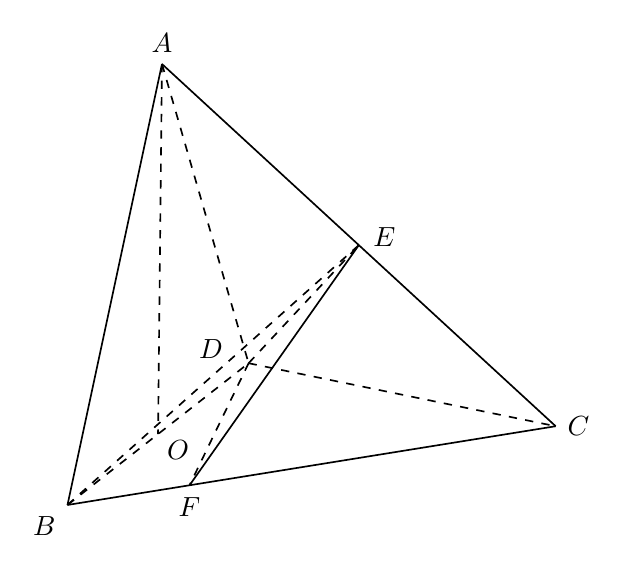
\begin{tikzpicture}[x=1cm,y=1cm,line width=.6pt,font=\normalsize,
  geometry edge/.style={solid,line width=.6pt},
  geometry label/.style={font=\normalsize,inner sep=2pt}]
\coordinate (B) at (0,0.2);
\coordinate (F) at (1.5500000000,0.4500000000);
\coordinate (C) at (6.2,1.2);
\coordinate (O) at (1.1500000000,1.1000000000);
\coordinate (D) at (2.3,2.0);
\coordinate (E) at (3.7000000000,3.5000000000);
\coordinate (A) at (1.2,5.8);
% solid outline + interior EF
\draw[geometry edge] (A)--(B);
\draw[geometry edge] (A)--(E)--(C);
\draw[geometry edge] (B)--(F)--(C);
\draw[geometry edge] (E)--(F);
% dashed base diagonals, altitude and interior segments
\draw[geometry edge,dashed] (B)--(E);
\draw[geometry edge,dashed] (D)--(C);
\draw[geometry edge,dashed] (B)--(D);
\draw[geometry edge,dashed] (D)--(E);
\draw[geometry edge,dashed] (D)--(F);
\draw[geometry edge,dashed] (A)--(O);
\draw[geometry edge,dashed] (A)--(D);
% labels with clearance
\node[geometry label,above] at ([yshift=2pt]A) {$A$};
\node[geometry label,below left] at ([xshift=-2pt,yshift=-2pt]B) {$B$};
\node[geometry label,right] at ([xshift=2pt]C) {$C$};
\node[geometry label,left,xshift=-5pt,yshift=5pt] at ([xshift=-2pt]D) {$D$};
\node[geometry label,right,xshift=1pt,yshift=3pt] at ([xshift=2pt]E) {$E$};
\node[geometry label,below] at ([yshift=-2pt]F) {$F$};
\node[geometry label,below right,xshift=-1.0pt,yshift=2pt] at ([xshift=2pt,yshift=-2pt]O) {$O$};
\end{tikzpicture}
